%%
%% This is file `sample-acmsmall.tex',
%% generated with the docstrip utility.
%%
%% The original source files were:
%%
%% samples.dtx  (with options: `acmsmall')
%% 
%% IMPORTANT NOTICE:
%% 
%% For the copyright see the source file.
%% 
%% Any modified versions of this file must be renamed
%% with new filenames distinct from sample-acmsmall.tex.
%% 
%% For distribution of the original source see the terms
%% for copying and modification in the file samples.dtx.
%% 
%% This generated file may be distributed as long as the
%% original source files, as listed above, are part of the
%% same distribution. (The sources need not necessarily be
%% in the same archive or directory.)
%%
%% The first command in your LaTeX source must be the \documentclass command.
 \documentclass[acmsmall]{acmart}

%%
%% \BibTeX command to typeset BibTeX logo in the docs
%%\AtBeginDocument{%
 %% \providecommand\BibTeX{{%
  %%  \normalfont B\kern-0.5em{\scshape i\kern-0.25em b}\kern-0.8em\TeX}}}

%% Rights management information.  This information is sent to you
%% when you complete the rights form.  These commands have SAMPLE
%% values in them; it is your responsibility as an author to replace
%% the commands and values with those provided to you when you
%% complete the rights form.



%%
%% These commands are for a JOURNAL article.
%% \acmJournal{JACM}
%% \acmVolume{37}
%% \acmNumber{4}
%% \acmArticle{111}

%%
%% Submission ID.
%% Use this when submitting an article to a sponsored event. You'll
%% receive a unique submission ID from the organizers
%% of the event, and this ID should be used as the parameter to this command.
%%\acmSubmissionID{123-A56-BU3}

%%
%% The majority of ACM publications use numbered citations and
%% references.  The command \citestyle{authoryear} switches to the
%% "author year" style.
%%
%% If you are preparing content for an event
%% sponsored by ACM SIGGRAPH, you must use the "author year" style of
%% citations and references.
%% Uncommenting
%% the next command will enable that style.
%%\citestyle{acmauthoryear}

%%
%% end of the preamble, start of the body of the document source.
\begin{document}

%%
%% The "title" command has an optional parameter,
%% allowing the author to define a "short title" to be used in page headers.
\title{Progetto 1 [SABD]}

%%
%% The "author" command and its associated commands are used to define
%% the authors and their affiliations.
%% Of note is the shared affiliation of the first two authors, and the
%% "authornote" and "authornotemark" commands
%% used to denote shared contribution to the research.
\author{Damiano Nardi}

\email{damiano6276@gmail.com}
\affiliation{%
 \institution{TorVergata, Corso Di Informatica}
 }

%%
%% By default, the full list of authors will be used in the page
%% headers. Often, this list is too long, and will overlap
%% other information printed in the page headers. This command allows
%% the author to define a more concise list
%% of authors' names for this purpose.

%%
%% The abstract is a short summary of the work to be presented in the

%\begin{abstract}

%\end{abstract}
%% article.

%%
%% The code below is generated by the tool at %%http://dl.acm.org/ccs.cfm.
%% Please copy and paste the code instead of the example below.
%%



%%
%% Keywords. The author(s) should pick words that accurately describe
%% the work being presented. Separate the keywords with commas.



%%
%% This command processes the author and affiliation and title
%% information and builds the first part of the formatted document.dsd
\maketitle{} 

\section{Introduzione}
In questa relazione si descriverà il lavoro svolto che consiste nella realizzazione delle query(1,2) e tutta l'infrastruttura  composta da vari framework istanziati su container docker per l'ingest, process e store dei dati.


\section{Processamento Delle Query}
Per processare le entrambe le query è stato usato il framework Spark usando le api java.

\subsection{Query1}
\begin{quote}
Per ogni settimana, calcolare il numero medio di guariti e dei tamponi effettuati in Italia in quella
settimana.\end{quote}

Una volta caricato il dataset come JavaRDD viene fatta una 

\subsubsection{flatMapToPair} 
in cui viene restituito 
come chiave il numero della settimana dell'anno e come valore una tupla composta da positivi,tamponi (vengono ignorati i giorni in mezzo alla settimana in base allo startingDay selezionato) successivamente viene fatto

\subsubsection{reduceByKey}
dove viene calcolata la media dei tamponi e guariti facendo la differenza dei giorni di inizio e fine settimana.
\subsubsection{ricreazione schema}
Viene poi ricreato lo schema e viene salvato il dataset processato in formato parquet su HDFS

\subsubsection{Tempi}
è stata tenuta traccia di due tempi: tempo di processamento della query e tempo del caricamento dello spark contex.

\hspace{40mm} \begin{tabular}{l|l|}
\cline{2-2}
                                       & tempo (sec.) \\ \hline
\multicolumn{1}{|l|}{Query processing} & 3            \\ \hline
\multicolumn{1}{|l|}{Spark loading}    & 5            \\ \hline
\end{tabular}

\subsection{Query2}
\begin{quote}
Per ogni continente, calcolare la media, la deviazione standard, il minimo e il massimo del numero di
casi confermati giornalmente per ogni settimana. Nel calcolo delle statistiche, considerare solo i 100
stati piu colpiti dalla pandemia. Qualora lo stato non fosse indicato, considerare la nazione. Per de- `
terminare gli stati piu colpiti nell’intero dataset, si consideri l’andamento degli incrementi giornalieri `
dei casi confermati attraverso il trendline coefficient. Per stimare il trendline coefficient, si calcoli la
pendenza della retta di regressione che approssima la tendenza degli incrementi giornalieri.
Nota: il continente a cui appartiene ogni nazione non viene indicato in modo esplicito nel dataset, ma
deve essere ricavato. Si considerino 6 continenti: Africa, America, Antartide, Asia, Europa, Oceania.\end{quote}

Una volta caricato il dataset come JavaRDD viene fatta una 
\subsubsection{flatMapToPair}
in cui la chiave è il coefficente di di tread line e il valore è un oggeto
"CovidGlob",all'interno ha la lista dei contagiati, la regione e la nazione, durante questa fase viene calcolato il coefficente di di tread line, la lista degli infetti per giorno viene trasformata da cumulativa alla lista dei nuovi casi per ogni giorno.
\subsubsection{top 100}
Vegono presi i top 100 stati con il coefficente di tread line più alto

\subsubsection{mapToPair}
La chiave vine cambiata dal coefficente di tread line alla nazione il valore rimane l'oggetto  "CovidGlob"

\subsubsection{Join}
Viene caricato come javaRDD un dataset esterno al progetto da HDFS preso da \\ \url{https://github.com/dbouquin/IS_608/blob/master/NanosatDB_munging/Countries-Continents.csv}   
essenziamelte è mapping continete-nazione, viene fatto un a mapToPair per rendere la nazione chiave e poi viene fatto il join con i top 100

\subsubsection{mapToPair}
Per rendere il continente key il valore invece è la lista degli infetti per giorno 
\subsubsection{reduceByKey}
per sommare le liste di infetti con lo stesso continente

\subsubsection{flatMap}
Per calcolare tutte le statistiche richieste per settimana, viene usata la flatMap in quanto da ogni RDD element verranno generate 4 liste:
lista delle medie,massimi,minimi,deviazioni standard tutte quante per settimana 
\subsubsection{ricreazione schema}
Viene poi ricreato lo schema e viene salvato il dataset processato in formato parquet su HDFS

\subsubsection{Tempi}
è stata tenuta traccia di due tempi: tempo di processamento della query e tempo del caricamento dello spark contex.

\hspace{40mm} \begin{tabular}{l|l|}
\cline{2-2}
                                       & tempo (sec.) \\ \hline
\multicolumn{1}{|l|}{Query processing} & 3            \\ \hline
\multicolumn{1}{|l|}{Spark loading}    & 5            \\ \hline
\end{tabular}


\section{INFRASTRUTTURA DI PROCESSAMENTO}
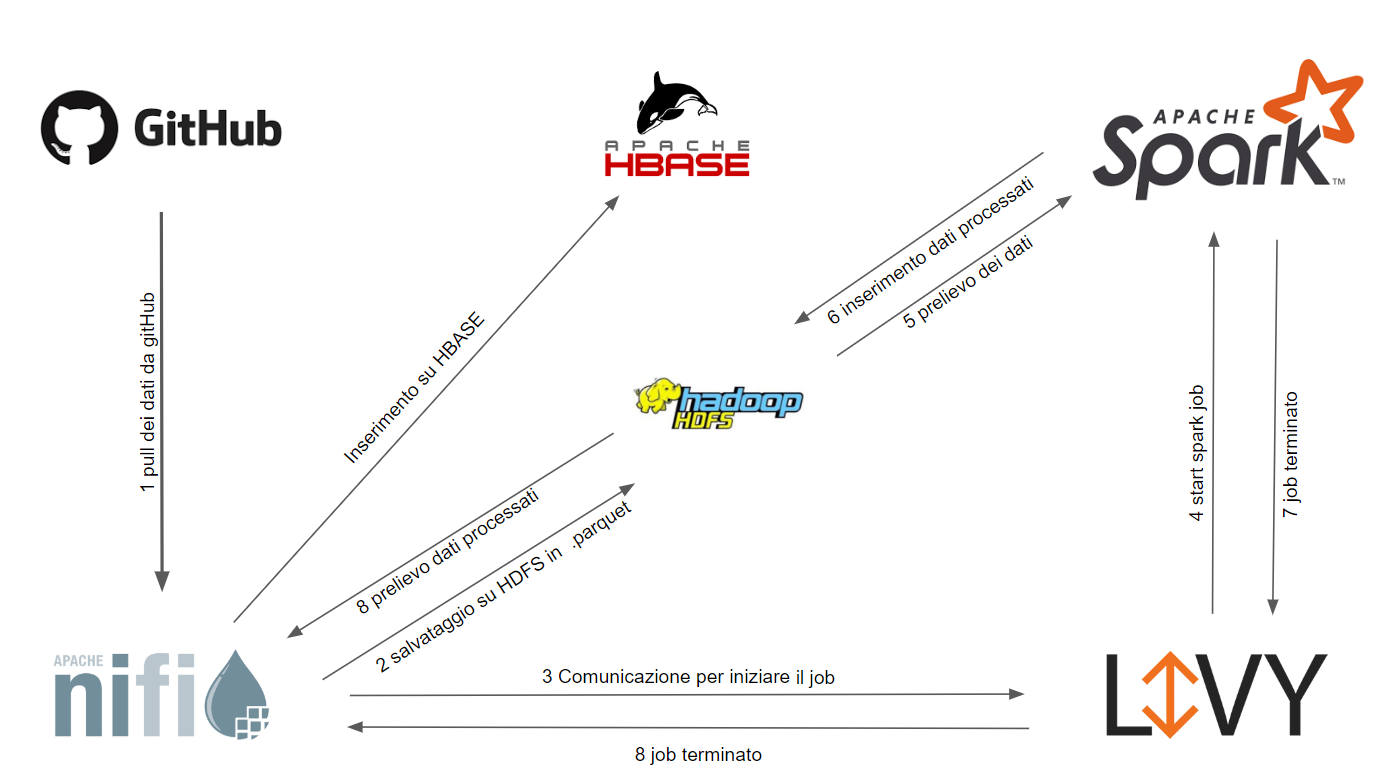
\includegraphics[width=14cm]{sistema.png}

\subsection{Framework utilizzati}

\subsubsection{Spark: processing} 
come visto prima si è utilizzato Spark per il processamento delle query, nello specifico è stato creato un cluster yarn composto da due worker e un master istanziati su container docker.


\subsubsection{NIFI: ingestion}
Si è utilizzato NiFi per fare data ingestion, nello specifico i dati vengono scaricati da gitHub ogni settimana, sono scremati attraverso una query sql, convertiti in formato parquet e caricati su HDFS (questo per la query1, Nifi non è riuscito a convertire in parquet il dataset della query2 quindi è stato caricato direttamente il csv per quest'ultima).
Di default Nifi non mette a disposizione un modo per comunicare con Spark, Livy viene in nostro (mio) aiuto permettendo a Nifi di inviare job a Spark e di sapere lo stato della computazione, in questo modo Nifi dopo aver finito l'upload dei dati su HDFS puo far iniziare a Spark il processamento e una volta finito Nifi può passare prelevare dati processati da HDFS e passarli al livello di storage \\ \\
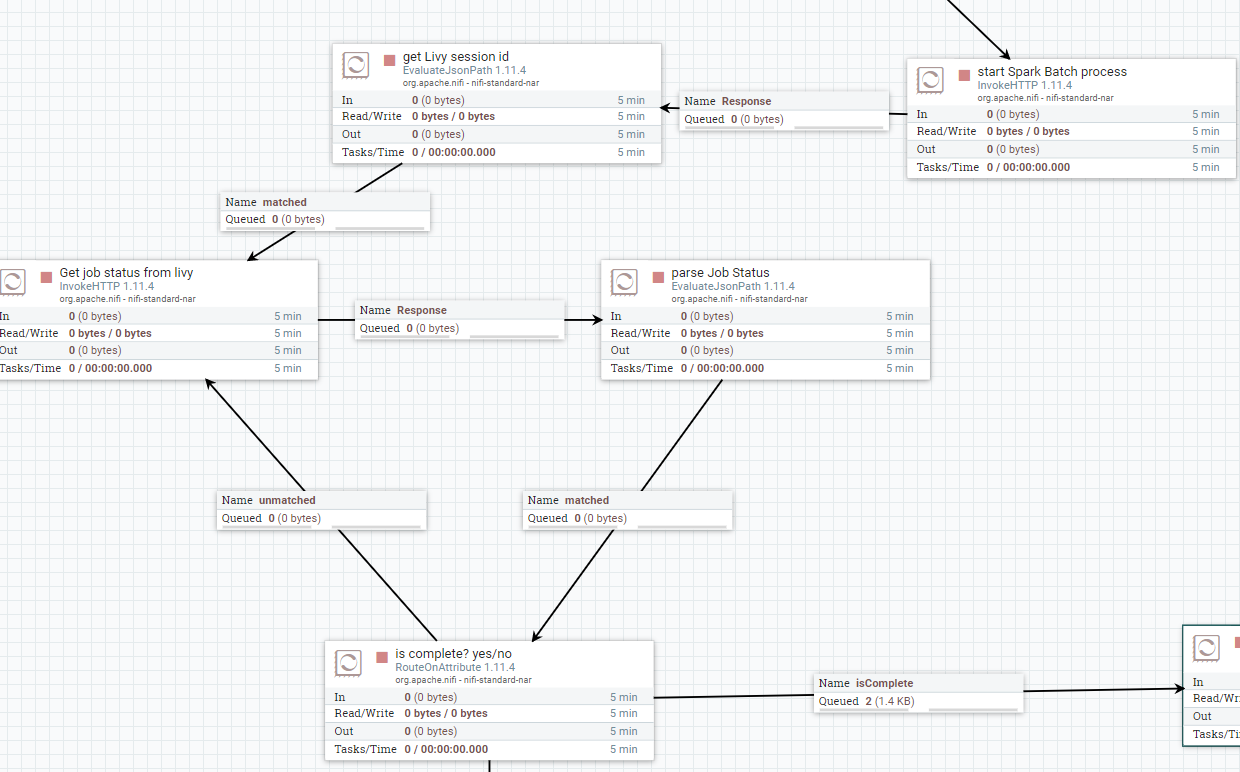
\includegraphics[width=14cm]{livy.png}
\\ \\

\subsubsection{Livy: layer di comunicazione}
Livy è un framework che mette a disposizione delle REST API per gestire Spark. In questo progetto è stato usato per far comunicare Nifi con Spark, nello specifico Nifi fa una post con dentro la classe main e la locazione del file jar nell' HDFS  da eseguire;
successivamente NiFi ogni 5 secondi controlla con una get a Livy lo stato del JoB, quando lo stato risulterà "succeed" Nifi continuerà il suo flusso 

\subsubsection{Hbase: Storage}
Per il layer di storage è stato utilizzato Hbase una volta che Spark ha finito la computazione Nifi si occupa di prendere i file parquet salvati 
da spark su HDFS processarli come parquet specificare la colonna che si vuole come key e caricarli su hbase.
Per la query1 come key è stata scelta la data (formato annoSettimana) in modo tale da ottimizzare lo scan inquanto i dati saranno memorizzati su posizioni vicine memoria, di contro qualora i dati dovessero diventare troppi si andrebbe a sovraccaricare un singolo region Server però considerata la quantità dei dati non è il caso.  Per la seconda query dopo il processamento abbiamo righe di questo tipo :
\\
\\
\hspace{1000mm}\begin{tabular}{|l|l|l|l|}
\hline
AAAEuropa  & europa  & MAX\_WEEK & ... \\ \hline
ZZZamerica & america & MIN\_WEEK & ... \\ \hline
IIIEuropa  & europa  & DEV\_WEEK & ... \\ \hline
RRREuropa  & europa  & AVG\_WEEK & ... \\ \hline
\end{tabular}
\\
\\
\\
 come key è stato scelto il campo della prima colonna, in questo modo le righe con la stessa funzione statica si troveranno sullo stesso regionserver e vicine tra loro ,andando ad ottimizare lo scan di tutti i continenti con una determinata funzione statistica 













\end{document}
\endinput
%%
%% End of file `sample-acmsmall.tex'.
